\documentclass{beamer} %% normal document
%\documentclass[notes]{beamer} %% notes in normal document
%\documentclass[draft,notes]{beamer} %% draft with notes
%\documentclass[handout]{beamer} %% handout

\usepackage{fontspec, unicode-math, caption}
\usepackage[ngerman]{babel}
\usepackage{graphicx}
\usepackage{float}
\usepackage{multicol}
\usepackage{listings}

%% usefull for handout with blank lines
%\usepackage{handoutWithNotes}
%\pgfpagesuselayout{2 on 1 with notes}[a4paper,border shrink=5mm]

%% usefull for presentation
%\setbeameroption{show notes on secondscreen=left}

\definecolor{bettergreen}{rgb}{.1,.7,.1}

\usetheme{Dresden}
\usecolortheme[named=bettergreen]{structure}
\useoutertheme{split}
\setbeamertemplate{caption}[numbered]
\captionsetup{labelformat=simple,font=scriptsize,labelfont=scriptsize}

% puts Frame numbers in Dresden template
\newcommand*\oldmacro{}%
\let\oldmacro\insertshorttitle%
\renewcommand*\insertshorttitle{%
	\oldmacro\hfill%
	\insertframenumber\,/\,\inserttotalframenumber}

\title[]{}

\author{
	Johannes Visintini, Philip Bell,\\
	Moritz Nöltner
}

\institute[IFI]{
	Vorlesung: Einführung in Software Engineering\\
	Institut für Informatik\\
	Universität Heidelberg
}
 
\begin{document}
\lstset{language=Java, showtabs=true, tabsize=2, breaklines=true,  breakatwhitespace=true,}

	\begin{frame}
		\titlepage
		\note{ }
	\end{frame}

	\section{Requirements}
	\subsection{Funktional}
	\begin{frame}{Requirements - Funktional}
		\textbf{UseCase}: SyncDialog\\
		\textit{Descripition}: öffnet sich wenn ein/e Abgleich/Aktualisierung\\
		\hspace{1em}oder der Use Case „Stichwortsuche (Filmtitel)“ aufgerufen wird\\
		\textit{Precondition}: Internetverbindung und MovieManager gestartet\\
		\textit{Postcondition}: Film wird vervollständigt/aktualisiert\\
		\textit{Exception}: Film in der Online-Datenbank nicht gefunden\\\vspace{1em}

		\textbf{UseCase}: Stichwortsuche (Filmtitel)\\
		\textit{Descripition}: Der User übergibt (über das Titel-Feld) ein
		Stichwort.\\\hspace{1em}Dann sucht das Programm nach diesem (oder
		ähnlichem) Titel \\\hspace{1em}in der Online-Datenbank.\\
		\textit{Precondition}: Internetverbindung und MovieManager gestartet\\
		\textit{Postcondition}: User bekommt Liste von Filmtiteln\\
		\textit{Exception}: kein Ergebnis gefunden
	\end{frame}

	\section{TestCases}
	\begin{frame}{TestCases}
		\begin{columns}[t]
			\begin{column}{.5\linewidth}
				\begin{figure}[H]
					\centering
					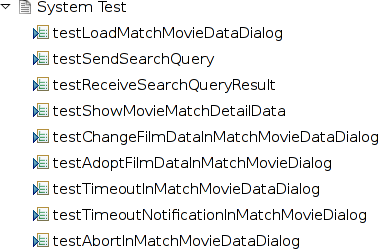
\includegraphics[width=\linewidth]{test-cases.png}
				\end{figure}
			\end{column}
			\begin{column}{.5\linewidth}
				\begin{figure}[H]
					\centering
					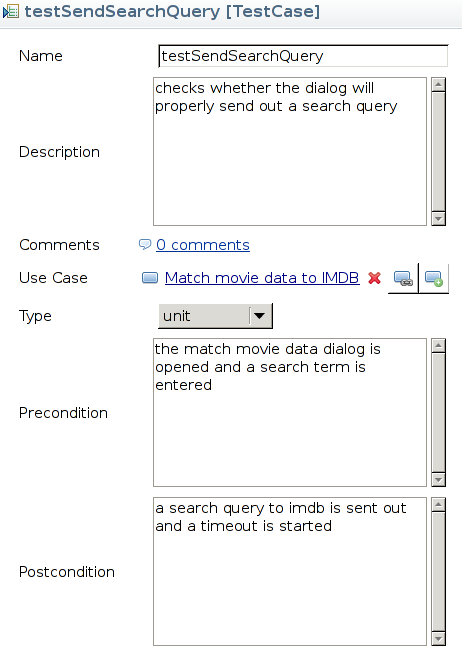
\includegraphics[height=.7\textheight]{testSendSearchQuery.png}
				\end{figure}
			\end{column}
		\end{columns}
	\end{frame}

	\section{GUI}
	\subsection{Entwurf}
	\begin{frame}{GUI - Entwurf}
		\begin{figure}[H]
			\centering
			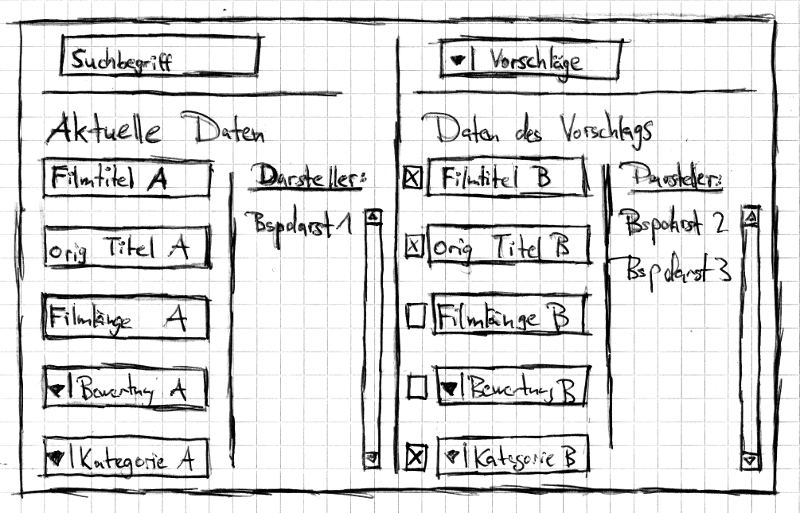
\includegraphics[width=\linewidth]{gui-mockup.png}
		\end{figure}
	\end{frame}

	\subsection{Show Loaned Movies Dialog}
	\begin{frame}{GUI - Show Loaned Movies Dialog}
		\begin{figure}[H]
			\centering
			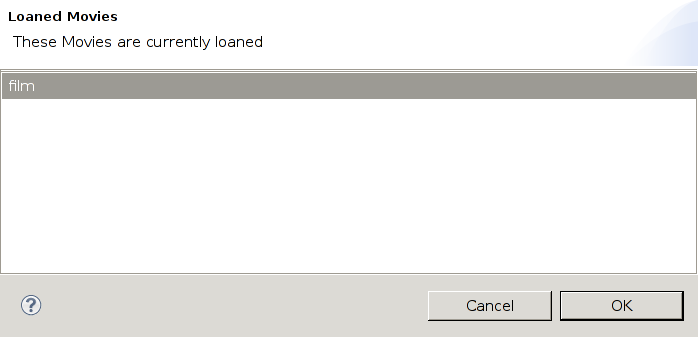
\includegraphics[width=\linewidth]{show-loaned-movies-dialog.png}
		\end{figure}
	\end{frame}

	\subsection{Add Performer Dialog}
	\begin{frame}{GUI - Add Performer Dialog}
		\begin{figure}[H]
			\centering
			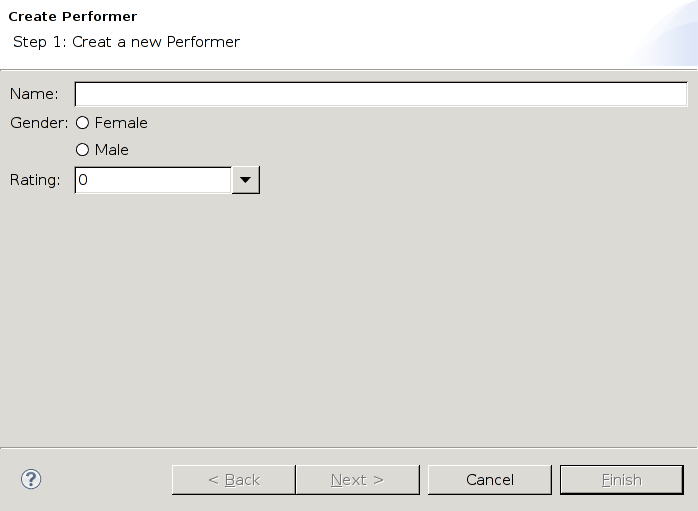
\includegraphics[width=\linewidth]{add-performer-dialog.png}
		\end{figure}
	\end{frame}

	\subsection{Movie Wizard}
	\begin{frame}{GUI - Movie Wizard}
		\begin{figure}[H]
			\centering
			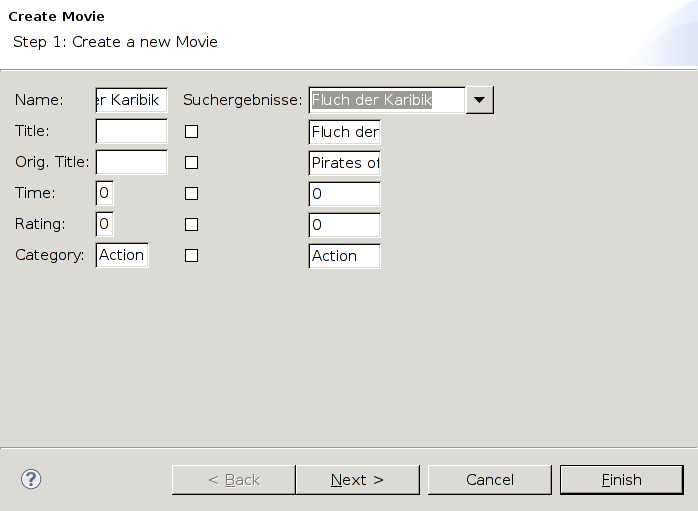
\includegraphics[width=\linewidth]{movie-wizard.png}
		\end{figure}
	\end{frame}

	\section{Implementation}
	\subsection{Query-Funktion}
	\begin{frame}[fragile]{Implementation - Query-Funktion}
		\tiny\begin{lstlisting}
suggestionDropDown.removeAll();
suggestionDropDown.select(0);
final String nearMovieName = textSearchName.getText(); 
Thread t = new Thread() {
    private void searchNearMovies(String title)
    {
        MovieQueryService mqs = new MovieQueryService();
        if (mqs.getListOfNearMovies(title) != null)
        {
            nearMovies = mqs.getListOfNearMovies(title);
        }
    }
    
    public void run()
    {
        searchNearMovies(nearMovieName);
        try {
            this.join();
        } catch (InterruptedException e) {
            e.printStackTrace();
        }
    }
};
t.start();
updateSuggestionDropDown();
setPageComplete(true);
		\end{lstlisting}
	\end{frame}

	\section{}
	\begin{frame}
		\center{\Huge ENDE}
	\end{frame}

\end{document}
